\documentclass[11pt,a4paper]{amsart}
\usepackage[T1]{fontenc}
\usepackage{lmodern,microtype}
\usepackage[margin=28mm]{geometry}
\usepackage{amsmath,amssymb,mathtools,booktabs,array,graphicx}
\usepackage{enumitem,tikz}
\usepackage[hidelinks]{hyperref}
\hypersetup{pdftitle={Domino tilings of odd-height rectangles up to symmetry},pdfauthor={Shiqi Liu}}
\newtheorem{theorem}{Theorem}[section]
\newtheorem{lemma}[theorem]{Lemma}
\newtheorem{proposition}[theorem]{Proposition}
\newtheorem{corollary}[theorem]{Corollary}
\theoremstyle{definition}
\newtheorem{definition}[theorem]{Definition}
\theoremstyle{remark}
\newtheorem{remark}[theorem]{Remark}
\newcommand{\Fix}{\operatorname{Fix}}
\newcommand{\Stab}{\operatorname{Stab}}
\newcommand{\rev}{\operatorname{rev}}
\newcommand{\one}{\boldsymbol{1}}
\newcommand{\evec}{e_0}
\newcommand{\trans}{\mathsf T}
\numberwithin{equation}{section}
\setlist{nosep}
\allowdisplaybreaks[2]
\title[Domino tilings up to symmetry]{Domino tilings of odd-height rectangles up to symmetry}
\author{Shiqi Liu}
\date{Version 2.0, October 25, 2026}
\subjclass[2020]{Primary 05A15; Secondary 05B45, 05A16}
\keywords{Domino tiling, Burnside's lemma, generating function, transfer matrix, symmetry class}
\begin{document}
\begin{abstract}
We count unlabelled domino tilings of odd-height rectangles of even width up to rectangle symmetries. For three rows, a block decomposition and a half-rectangle construction give the generating function recorded in OEIS A232622, its seventh-order recurrence, and all initial values. We also give stabilizer and asymptotic formulas, an odd-height transfer expression, and an explicit five-row polynomial certificate. The three-row main counting theorem has Lean M1--M6 evidence based on actual tiling-orbit cardinalities. This edition explains the state induction and the four coefficients of the compressed recurrence in detail. The formal coverage reported here is limited to M1--M6; external semantic review and bibliographic priority remain unresolved.
\end{abstract}
\maketitle
\noindent\textbf{Scope of this edition.}
Theorem \ref{thm:main} and its three-row half-rectangle dependencies
have the M1--M6 formal evidence described in Section \ref{sec:formalization}.
This edition reports that fixed scope, rather than a certification of
all results in the manuscript. Independent mathematical and semantic
review remain outstanding, and no bibliographic priority is claimed.
\medskip

\section{Introduction}\label{sec:intro}

Let $\mathcal T_n$ be the set of domino tilings of a $3\times 2n$
rectangle, where $n\ge1$. A domino covers two unit cells sharing an
edge. Both orientations are allowed, the dominoes are unlabelled,
and no tatami restriction is imposed. Thus a tiling is a set of
unordered pairs of adjacent cells.
Number rows from top to bottom and columns from left to right.
The maps
\[
 h(r,c)=(4-r,c),\qquad v(r,c)=(r,2n+1-c),\qquad \rho=hv
\]
are reflection in the horizontal axis, reflection in the vertical
axis, and rotation through $180^\circ$, respectively.
Since $3\ne2n$, the full symmetry group of the rectangle is
$G=\{e,h,v,\rho\}\cong C_2\times C_2$.
Write $a(n)=|\mathcal T_n/G|$. We set $\mathcal T_0$ to consist of a
single empty tiling, fixed by all four abstract group elements, so
that $a(0)=1$.

Mathar \cite[Table 10, Conjecture 6]{mathar2013} proposed a generating
function for these symmetry classes. The equivalent formula in
OEIS A232622 \cite{oeis} is accompanied by a conjectured recurrence
of order seven. We give two derivations, with the M1--M6 formal evidence following the half-rectangle route.
The first uses a complete classification of vertically
indecomposable blocks and the action of $G$ on words in these blocks.
The second counts symmetric tilings directly from partial tilings
of a half-rectangle.
The latter construction also yields a uniform formula for any fixed
odd height.

Transfer matrices and indecomposable tilings are established tools
in fixed-width enumeration. In particular, Mathar
\cite[Sections 2.1--2.3]{mathar2014} gives the ordinary three-row
generating function and the corresponding indecomposable-block
generating function. We rederive the required block classification
and determine the symmetry action explicitly.
DeFord \cite[Theorem 6.1]{deford} establishes a general recurrence
framework for rectangular tilings counted up to symmetry and
illustrates it for two-row domino tilings in Section 6.2.1.
Thus rationality at fixed height is established background;
our odd-height formula specifies the boundary conditions and
gives an explicit five-row evaluation.
None of our
combinatorial arguments assumes the target recurrence or a finite
list of coefficients.
The source entry was checked on October 25, 2026; its conjecture
label does not establish that no equivalent proof appears elsewhere.
No claim of bibliographic priority is made here.

\paragraph{Reading the widths and counts.}
The exponent $n$ always records half the full width $2n$.
In Section \ref{sec:half}, $q_w(S)$ counts a partial rectangle of
actual width $w$, while the induction index $j$ groups widths $2j$
and $2j+1$. Thus $\alpha_j=q_{2j}(\varnothing)=d_j$, whereas
$\beta_j=q_{2j}(\{1,2\})$ counts one terminal state.
The full transfer uses row vectors; its two-coordinate compression
in \eqref{eq:two-dimensional} uses column vectors.

\subsection{Main result}
Let
\[
 d_n=|\mathcal T_n|,\qquad h_n=|\Fix(h)|,\qquad
 v_n=|\Fix(v)|,\qquad r_n=|\Fix(\rho)|.
\]
Their ordinary generating functions, with $x$ marking the
half-width $n$, are denoted by $D,H,V,R$.
All generating-function identities are interpreted in
$\mathbb Q[[x]]$.

\begin{theorem}\label{thm:main}
The number of domino tilings of a $3\times2n$ rectangle up to
rectangle symmetries has generating function
\begin{equation}\label{eq:main}
 A(x):=\sum_{n\ge0}a(n)x^n
 =\frac{1-3x-4x^2+10x^3-4x^5+x^6}
 {(1-x)(1-4x+x^2)(1-4x^2+x^4)}.
\end{equation}
Consequently,
\begin{equation}\label{eq:recurrence}
\begin{split}
a(n)={}&5a(n-1)-a(n-2)-19a(n-3)+19a(n-4)\\
       &+a(n-5)-5a(n-6)+a(n-7),\qquad n\ge7,
\end{split}
\end{equation}
with initial values
\[
 (a(0),\ldots,a(6))=(1,2,5,14,46,156,561).
\]
\end{theorem}

Multiplying the numerator and denominator in \eqref{eq:main} by
$-1$ gives the form displayed in A232622.
Sections \ref{sec:blocks} and \ref{sec:half} give the two proofs.
Section \ref{sec:types} determines the exact stabilizers and the
asymptotic proportion of symmetric tilings.
Sections \ref{sec:odd} and \ref{sec:five} treat arbitrary odd height
and the explicit five-row case.

\begin{lemma}[Burnside's formula]\label{lem:burnside}
For every $n\ge0$,
\begin{equation}\label{eq:burnside}
 a(n)=\frac{d_n+h_n+v_n+r_n}{4}.
\end{equation}
\end{lemma}
\begin{proof}
Count the pairs $(g,T)\in G\times\mathcal T_n$ with $gT=T$:
\[
 \sum_{g\in G}|\Fix(g)|
 =\sum_{T\in\mathcal T_n}|\Stab(T)|.
\]
By the orbit--stabilizer formula, each orbit $O$ contributes
$|O|\cdot4/|O|=4$ to the right-hand side.
Division by four proves the assertion.
This is the usual orbit-counting lemma; see
\cite[Chapter 7, Lemma 7.2]{stanley}.
The argument does not require a faithful action and includes $n=0$.
\end{proof}

\section{Indecomposable blocks}\label{sec:blocks}

\subsection{Column states}
Consider a three-row rectangle of arbitrary width $w$.
At the cut between columns $j$ and $j+1$, let
$S_j\subseteq\{1,2,3\}$ be the set of rows crossed by a horizontal
domino. Set $S_0=S_w=\varnothing$.
If a column has incoming state $p$ and outgoing state $q$, then
the transition is legal precisely when
\begin{equation}\label{eq:local3}
 p\cap q=\varnothing,\qquad
 \{1,2,3\}\setminus(p\cup q)\in
 \{\varnothing,\{1,2\},\{2,3\}\}.
\end{equation}
Indeed, the cells in $p$ are covered from the left, those in $q$
are covered towards the right, and the remaining cells must be
paired vertically. Their vertical completion is unique.
Table \ref{tab:states} lists every transition.

\begin{table}[htbp]
\centering
\caption{The complete three-row transition table.}\label{tab:states}
\begin{tabular}{cc@{\qquad}cc}
\toprule
Input & Outputs & Input & Outputs\\
\midrule
$\varnothing$ & $\{1\},\{3\},\{1,2,3\}$ &
$\{1,2\}$ & $\{3\}$\\
$\{1\}$ & $\varnothing,\{2,3\}$ &
$\{1,3\}$ & $\{2\}$\\
$\{2\}$ & $\{1,3\}$ &
$\{2,3\}$ & $\{1\}$\\
$\{3\}$ & $\varnothing,\{1,2\}$ &
$\{1,2,3\}$ & $\varnothing$\\
\bottomrule
\end{tabular}
\end{table}

\begin{lemma}\label{lem:path}
Tilings of a $3\times w$ rectangle are in bijection with legal
state paths of length $w$ from $\varnothing$ to $\varnothing$.
\end{lemma}
\begin{proof}
A tiling determines its cut states uniquely.
Conversely, place a horizontal domino at every row specified by
each internal cut state, and fill the remaining cells in each
column with the unique vertical completion.
Condition \eqref{eq:local3} prevents overlapping horizontal
dominoes and ensures that every remaining cell is covered.
The empty endpoint states exclude dominoes extending beyond the
rectangle. These constructions are inverse to one another.
The empty path gives the empty tiling when $w=0$.
\end{proof}

\subsection{First returns and block classification}
\begin{definition}
An internal vertical grid line crossed by no domino is a
\emph{fault}. A nonempty tiling of a three-row rectangle is an
\emph{indecomposable block} if it has no internal fault.
\end{definition}

\begin{lemma}\label{lem:blocks}
The indecomposable blocks are exactly $C$ and $A_k,B_k$ for $k\ge1$.
Here $C$ is the width-two block consisting of three horizontal
dominoes. The block $A_k$ has width $2k$ and consists of:
\begin{enumerate}
\item vertical dominoes in columns $1$ and $2k$, each covering
rows $1$ and $2$;
\item horizontal dominoes in row $3$ on column pairs
$(2j-1,2j)$, where $1\le j\le k$;
\item horizontal dominoes in each of rows $1,2$ on column pairs
$(2j,2j+1)$, where $1\le j<k$.
\end{enumerate}
The block $B_k$ is the horizontal-axis reflection $h(A_k)$.
\end{lemma}
\begin{proof}
By Lemma \ref{lem:path}, a block is a first-return path from the
empty state. Its first step has three possibilities.
If it reaches $\{1,2,3\}$, the next step is forced back to
$\varnothing$, giving $C$.
If it reaches $\{3\}$, every nonterminal excursion consists of
the two steps
$\{3\}\to\{1,2\}\to\{3\}$.
After $k-1$ such excursions, the path returns from $\{3\}$ to
$\varnothing$. This is a path of length $2k$ and gives exactly
the stated coordinates of $A_k$.
If the first step reaches $\{1\}$, the corresponding excursions
are $\{1\}\to\{2,3\}\to\{1\}$, giving $B_k$.
The complete transition table allows no other first-return path.

Every listed block is indeed indecomposable.
In $A_k$, every odd internal cut is crossed by a domino in row
$3$, and every even internal cut is crossed by dominoes in rows
$1,2$. Reflection gives the same assertion for $B_k$.
The unique internal cut of $C$ is crossed in all three rows.
The position of the first vertical domino distinguishes $A_k$
from $B_k$, whereas $C$ has no vertical domino.
Thus the classification has neither omissions nor repetitions.
\end{proof}

\begin{figure}[htbp]
\centering
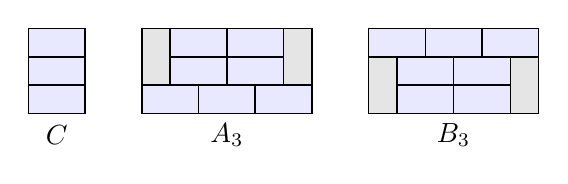
\begin{tikzpicture}[x=0.36cm,y=0.36cm,line width=0.55pt]
\begin{scope}
 \foreach \y in {0,1,2}{\draw[fill=blue!9] (0,\y) rectangle ++(2,1);}
 \node at (1,-0.75) {$C$};
\end{scope}
\begin{scope}[shift={(4,0)}]
 \draw[fill=gray!20] (0,1) rectangle (1,3);
 \draw[fill=gray!20] (5,1) rectangle (6,3);
 \foreach \x in {0,2,4}{\draw[fill=blue!9] (\x,0) rectangle ++(2,1);}
 \foreach \y in {1,2}{\foreach \x in {1,3}{\draw[fill=blue!9] (\x,\y) rectangle ++(2,1);}}
 \node at (3,-0.75) {$A_3$};
\end{scope}
\begin{scope}[shift={(12,0)}]
 \draw[fill=gray!20] (0,0) rectangle (1,2);
 \draw[fill=gray!20] (5,0) rectangle (6,2);
 \foreach \x in {0,2,4}{\draw[fill=blue!9] (\x,2) rectangle ++(2,1);}
 \foreach \y in {0,1}{\foreach \x in {1,3}{\draw[fill=blue!9] (\x,\y) rectangle ++(2,1);}}
 \node at (3,-0.75) {$B_3$};
\end{scope}
\end{tikzpicture}

\caption{Representative blocks $C,A_3,B_3$. Rectangle boundaries
are domino boundaries. The diagram was drawn from the coordinate
definitions using AI-assisted TikZ code.}\label{fig:blocks}
\end{figure}

\begin{lemma}\label{lem:word}
Every three-row tiling has a unique decomposition into a word
over $\mathcal B=\{C\}\cup\{A_k,B_k:k\ge1\}$.
Let $\sigma$ fix $C$ and interchange $A_k,B_k$.
Under this correspondence,
\begin{equation}\label{eq:word-action}
 h(W)=\sigma(W),\qquad v(W)=\rev(W),\qquad
 \rho(W)=\sigma(\rev(W)),
\end{equation}
where $\sigma$ is applied letterwise.
\end{lemma}
\begin{proof}
Cut a tiling at all its faults. The resulting pieces have no
internal faults and hence are precisely the blocks of Lemma
\ref{lem:blocks}. Every boundary in a block decomposition must
be a fault, and every fault must be used: omitting one would
leave a decomposable piece. This proves uniqueness.
Concatenation gives the inverse map, with the empty word
corresponding to the empty tiling.

Horizontal-axis reflection acts on individual blocks by $\sigma$.
Every block is invariant under vertical-axis reflection.
For $A_k$, the column reversal $c\mapsto2k+1-c$ interchanges
the endpoint vertical dominoes. It sends each bottom-row pair
$(2j-1,2j)$ to another such pair, with index $k+1-j$,
and each upper-row pair $(2j,2j+1)$ to another, with index $k-j$.
The block $C$ is fixed domino by domino. Since the two
reflections commute and $B_k=h(A_k)$, every $B_k$ is also
invariant under vertical-axis reflection.

Both reflections preserve the set of faults. Horizontal-axis
reflection preserves block order, whereas vertical-axis
reflection reverses it. Uniqueness of the decomposition now
gives \eqref{eq:word-action}, including when block widths differ.
\end{proof}

\subsection{Fixed words}
Assign weight $x$ to $C$ and $x^k$ to $A_k,B_k$.
The exponent records half the width.
The block generating function is
\begin{equation}\label{eq:F}
 F(x)=x+2\sum_{k\ge1}x^k=\frac{3x-x^2}{1-x}.
\end{equation}
Since $F(0)=0$, only finitely many words contribute to any
given coefficient.

\begin{proposition}\label{prop:fixed-gf}
The four fixed-point generating functions are
\begin{align}
D(x)&=\frac{1}{1-F(x)}=\frac{1-x}{1-4x+x^2},
&H(x)&=\frac{1}{1-x},\label{eq:DH}\\
V(x)&=(1+F(x))D(x^2)
 =\frac{1+3x+x^2-x^3}{1-4x^2+x^4},\label{eq:V}\\
R(x)&=(1+x)D(x^2)
 =\frac{1+x-x^2-x^3}{1-4x^2+x^4}.\label{eq:R}
\end{align}
\end{proposition}
\begin{proof}
An arbitrary word contributes to
$D=\sum_{\ell\ge0}F^\ell$.
A word fixed by $h$ must consist entirely of letters fixed by
$\sigma$. The only such letter is $C$, giving $H$.

A word fixed by $v$ is a palindrome. It has a unique expression
$U\rev(U)$ or $Ub\rev(U)$, where $b$ is any block.
The two copies of $U$ contribute $D(x^2)$, and the possible
central block contributes $1+F(x)$.

A word fixed by $\rho$ has a unique expression
$U\sigma(\rev(U))$, or $Ub\sigma(\rev(U))$ with $\sigma(b)=b$.
In the latter case $b=C$, so the central contribution is $1+x$.
In both constructions the two cases are disjoint and the
decomposition is reversible. A central block may cross the
geometric midline; that line is not required to be a fault.
\end{proof}

\begin{proof}[First proof of Theorem \ref{thm:main}]
Burnside's formula and Proposition \ref{prop:fixed-gf} give
\begin{equation}\label{eq:average-rational}
 A(x)=\frac14\left[
 \frac{1-x}{1-4x+x^2}+\frac1{1-x}
 +\frac{2(1+2x-x^3)}{1-4x^2+x^4}\right].
\end{equation}
Put $P_3=1-4x+x^2$ and $Q_3=1-4x^2+x^4$.
On taking the common denominator $(1-x)P_3Q_3$, its numerator is
\begin{align*}
 &\frac{(1-x)^2Q_3+P_3Q_3+
 2(1+2x-x^3)(1-x)P_3}{4}\\
 &\hspace{35mm}=1-3x-4x^2+10x^3-4x^5+x^6.
\end{align*}
This proves \eqref{eq:main}. The denominator expands to
\[
 1-5x+x^2+19x^3-19x^4-x^5+5x^6-x^7.
\]
The numerator has degree six, so comparison of coefficients
of $x^n$ for $n\ge7$ gives \eqref{eq:recurrence}.
The coefficients of degrees zero through six give the initial
values in the theorem.
\end{proof}

\begin{remark}
In \cite[equation (26)]{mathar2013}, the variable $z$ marks the
full width, so the appropriate comparison is
$\overline T(z,3)=A(z^2)$.
After substitution into \eqref{eq:average-rational}, the
horizontal-reflection contribution $H(z^2)/4$ can be written as
\[
 \frac18\left(\frac1{1+z}+\frac1{1-z}\right)
 =\frac1{4(1-z^2)},
\]
Rearranging the other contributions gives the cited expression.
In the three-row formulas of
\cite[equations (4)--(6)]{mathar2014}, $z$ instead marks the
number of dominoes; the corresponding substitution is $z^3=x$.
\end{remark}

\section{Half-rectangle bijections}\label{sec:half}
We now derive the fixed-point counts without using the block
classification or the palindrome argument. The local construction
is stated for any positive height.

\subsection{Partial tilings and a transfer matrix}
For $m,j\ge1$ and $S\subseteq[m]=\{1,\ldots,m\}$,
let $\mathcal P_m(j,S)$ be the set of partial tilings of an
$m\times j$ rectangle that cover every cell except the cells in
rows $S$ of the last column.
Each uncovered cell is regarded as the left half of a horizontal
domino to be completed in the next column.
For $j=0$, only the empty object with $S=\varnothing$ is allowed.
Write $q_j(S)=|\mathcal P_m(j,S)|$.

Index rows and columns of $T_m$ by all subsets of $[m]$, and set
\begin{equation}\label{eq:Tm}
 T_m[p,q]=
 \begin{cases}
 1,&p\cap q=\varnothing\ \text{and every consecutive run}\\
   &\quad\text{in }[m]\setminus(p\cup q)\text{ has even length},\\
 0,&\text{otherwise}.
 \end{cases}
\end{equation}
An empty complement satisfies the condition.
The cells in $p$ complete the incoming horizontal dominoes;
those in $q$ remain as outgoing halves.
Each remaining consecutive run has a vertical tiling if and
only if its length is even, and then that tiling is unique.
This follows by pairing the endpoint with its only available
neighbour and proceeding along the run.
Consequently, legal state paths and partial tilings determine
one another uniquely.

Let $\evec$ be the unit column vector at the empty state, and
let $t_m(j)$ count complete $m\times j$ tilings. Then
\begin{equation}\label{eq:profile}
 q_j^{\trans}=\evec^{\trans}T_m^j,\qquad
 t_m(j)=\evec^{\trans}T_m^j\evec.
\end{equation}
For an auxiliary height-zero term, set $T_0=(1)$ and $t_0(j)=1$.

\subsection{Boundary conditions imposed by symmetry}
Define $J(S)=\{m+1-r:r\in S\}$.
Let $\one$ be the all-ones column vector, and let
$\chi_m(S)=1$ if $J(S)=S$, and $0$ otherwise.
Denote the fixed-point counts of the two reflections and the
half-turn on an $m\times2n$ rectangle by $h_{m,n},v_{m,n},r_{m,n}$,
respectively.

\begin{lemma}\label{lem:half}
For every $m\ge1$ and $n\ge0$,
\begin{equation}\label{eq:half-fixed}
 v_{m,n}=\evec^{\trans}T_m^n\one,\qquad
 r_{m,n}=\evec^{\trans}T_m^n\chi_m.
\end{equation}
\end{lemma}
\begin{proof}
Suppose first that $n\ge1$. Given $P\in\mathcal P_m(n,S)$,
reflect its internal dominoes into the right half of the
rectangle, and insert a horizontal domino joining $(r,n)$
to $(r,n+1)$ for each $r\in S$.
The internal dominoes in the two halves are disjoint, and the
inserted dominoes cover precisely the remaining cells.
The resulting tiling is fixed by vertical-axis reflection.
Conversely, restrict any such fixed tiling to its left half
and cut its midline-crossing dominoes. This recovers $P,S$
uniquely, proving the first bijection and formula.

For the half-turn, rotate the internal dominoes of $P$ into
the right half. The unmatched rows on the right are $J(S)$.
A domino crossing the midline must join two cells in the same
row, so completion is possible if and only if $J(S)=S$.
When this condition holds, inserting one crossing domino in
each row of $S$ gives a half-turn-invariant tiling.
Restriction to the left half is again the inverse map.
Equivalently, necessity follows because the half-turn sends a
crossing domino in row $r$ to one in row $m+1-r$.
The empty-object convention gives both formulas for $n=0$.
\end{proof}

\begin{lemma}\label{lem:h-odd}
If $m=2k+1$ with $k\ge0$, then
\begin{equation}\label{eq:h-odd}
 h_{m,n}=t_k(2n)\qquad(n\ge0).
\end{equation}
\end{lemma}
\begin{proof}
In a tiling fixed by horizontal-axis reflection, a vertical
domino incident with the middle row would have a distinct
reflected image sharing its middle-row cell. Such a domino
is impossible.
The middle row must therefore have its unique horizontal
tiling. The top $k$ rows form a complete tiling, and their
reflection determines the bottom $k$ rows.
Conversely, every tiling of the top subrectangle gives a fixed
tiling in this way. Restriction is the inverse.
The conventions cover $k=0$ and $n=0$.
\end{proof}

\subsection{A two-dimensional recurrence for height three}
From \eqref{eq:Tm}, the states reachable from the empty state
at height three are
\[
\varnothing,\quad\{1\},\quad\{3\},\quad\{1,2\},\quad\{2,3\},\quad\{1,2,3\}.
\]
The empty state leads to $\{1\},\{3\},\{1,2,3\}$;
$\{1\}$ leads to $\varnothing,\{2,3\}$;
$\{3\}$ leads to $\varnothing,\{1,2\}$;
The remaining transitions are
\[
\{1,2\}\longrightarrow\{3\},\qquad
\{2,3\}\longrightarrow\{1\},\qquad
\{1,2,3\}\longrightarrow\varnothing.
\]
We now make the induction explicit. Put
\[
 E=\{\varnothing,\{1,2\},\{2,3\}\},\qquad
 O=\{\{1\},\{3\},\{1,2,3\}\}.
\]
Every transition out of $E$ ends in $O$, and every transition out of
$O$ ends in $E$. There is no exit to either of the other two states.
This is a statement about the complete list of allowed exits, not a
claim that every pair of states in the two sets is connected.

\paragraph{Induction statement and base case.}
For each $j\ge0$, the support of $q_{2j}$ is contained in $E$, and
\[
 q_{2j}(\varnothing)=\alpha_j,\qquad
 q_{2j}(\{1,2\})=q_{2j}(\{2,3\})=\beta_j.
\]
Thus $\beta_j$ counts one specified state; the two nonempty states
together contribute $2\beta_j$. We do not assert that all states of
$E$ have positive counts. At width zero only the empty state occurs,
so $(\alpha_0,\beta_0)=(1,0)$, including equality of the two zero counts.

\paragraph{One added column.}
Assume the statement at width $2j$. Grouping by the previous state gives
\[
\begin{aligned}
q_{2j+1}(\{1\})
 &=q_{2j}(\varnothing)+q_{2j}(\{2,3\})=\alpha_j+\beta_j,\\
q_{2j+1}(\{3\})
 &=q_{2j}(\varnothing)+q_{2j}(\{1,2\})=\alpha_j+\beta_j,\\
q_{2j+1}(\{1,2,3\})&=q_{2j}(\varnothing)=\alpha_j.
\end{aligned}
\]
All other counts are zero because the exits from $E$ have been exhausted.
Each legal transition has exactly one local filling. Conversely,
removing the added column, and cutting any horizontal domino crossing
its left boundary, recovers a unique previous object and state.
The source classes are therefore disjoint and exhaustive; no extra
multiplicity is needed in these sums.

\paragraph{A second added column.}
All three states in $O$ can end at the empty state. Only $\{3\}$
can end at $\{1,2\}$, and only $\{1\}$ can end at $\{2,3\}$.
Consequently,
\[
\begin{aligned}
q_{2j+2}(\varnothing)
 &=q_{2j+1}(\{1\})+q_{2j+1}(\{3\})+q_{2j+1}(\{1,2,3\})\\
 &=(\alpha_j+\beta_j)+(\alpha_j+\beta_j)+\alpha_j
   =3\alpha_j+2\beta_j,\\
q_{2j+2}(\{1,2\})&=q_{2j+1}(\{3\})=\alpha_j+\beta_j,\\
q_{2j+2}(\{2,3\})&=q_{2j+1}(\{1\})=\alpha_j+\beta_j.
\end{aligned}
\]
There are no other nonzero counts, since all exits from $O$ lie in $E$.
This proves the support statement and equality of the two counts at
the next even width, completing the induction for every $j\ge0$.
In column-vector form the recurrence is
\begin{equation}\label{eq:two-dimensional}
 \binom{\alpha_{j+1}}{\beta_{j+1}}
 =\begin{pmatrix}3&2\\1&1\end{pmatrix}
 \binom{\alpha_j}{\beta_j},\qquad
 (\alpha_0,\beta_0)=(1,0).
\end{equation}

\paragraph{Reading the four coefficients.}
The first row counts arrivals at $\varnothing$; the second counts
arrivals at the single target $\{1,2\}$.
\begin{center}
\small
\begin{tabular}{cp{0.78\linewidth}}
\toprule
Entry & Two-column continuation counted\\
\midrule
$3$ & From $\varnothing$ back to $\varnothing$, through any of
$\{1\}$, $\{3\}$, or $\{1,2,3\}$.\\
$2$ & One return to $\varnothing$ from each of $\{1,2\}$ and
$\{2,3\}$, giving two source classes of size $\beta_j$.\\
$1$ & From $\varnothing$ through $\{3\}$ to $\{1,2\}$.\\
$1$ & From $\{1,2\}$ through $\{3\}$ back to $\{1,2\}$;
the other nonempty state contributes nothing to this target.\\
\bottomrule
\end{tabular}
\end{center}
In particular, the coefficient $2$ does not mean that each object
in a fixed nonempty state has two returns to the empty state.
For example, $(\alpha_1,\beta_1)=(3,1)$ gives
$\alpha_2=(3+1)+(3+1)+3=11$ and $\beta_2=3+1=4$.
This example illustrates the induction; it is not its basis.

\begin{proposition}\label{prop:parity}
The ordinary counts $d_j=t_3(2j)$ satisfy
\begin{equation}\label{eq:d-rec}
 d_0=1,\qquad d_1=3,\qquad
 d_{j+2}=4d_{j+1}-d_j\quad(j\ge0).
\end{equation}
For every $j\ge0$,
\begin{equation}\label{eq:parity-fixed}
\begin{gathered}
 h_n=1\quad(n\ge0),\qquad r_{2j}=r_{2j+1}=d_j,\\
 v_{2j}=d_{j+1}-2d_j,\qquad v_{2j+1}=d_{j+1}.
\end{gathered}
\end{equation}
In particular,
\begin{equation}\label{eq:parity-orbits}
\begin{split}
 a(2j)&=\frac{d_{2j}+1+d_{j+1}-d_j}{4},\\
 a(2j+1)&=\frac{d_{2j+1}+1+d_{j+1}+d_j}{4}.
\end{split}
\end{equation}
\end{proposition}
\begin{proof}
Equation \eqref{eq:profile} gives $d_j=\alpha_j$.
The matrix in \eqref{eq:two-dimensional} satisfies
$M^2-4M+I=0$, proving \eqref{eq:d-rec}.
At an even step, the only reachable $J$-invariant state is
$\varnothing$; at an odd step it is $\{1,2,3\}$.
Lemma \ref{lem:half} therefore gives the two formulas for $r$.
Summing all terminal counts gives
$\alpha_j+2\beta_j=d_{j+1}-2d_j$ at an even step and
$3\alpha_j+2\beta_j=d_{j+1}$ at an odd step.
Lemma \ref{lem:h-odd} gives $h_n=t_1(2n)=1$.
Substitution in Burnside's formula proves \eqref{eq:parity-orbits}.
\end{proof}

\begin{proof}[Second proof of Theorem \ref{thm:main}]
The recurrence \eqref{eq:d-rec} gives
$D(x)=(1-x)/(1-4x+x^2)$.
Summing \eqref{eq:parity-fixed} over the two parities gives
\[
 H(x)=\frac1{1-x},\qquad R(x)=(1+x)D(x^2),
\]
and
\[
 V(x)=(1+x)\frac{D(x^2)-1}{x^2}-2D(x^2)
 =\frac{1+3x+x^2-x^3}{1-4x^2+x^4}.
\]
The quotient denotes the unique coefficient shift: $D(t)-1=tE(t)$, where $E(t)=\sum_{j\ge0}d_{j+1}t^j$. It does not treat $t$ as a unit in the formal power-series ring.
Burnside's formula now gives \eqref{eq:average-rational};
the algebraic simplification and coefficient comparison in
the first proof finish the argument.
The combinatorial derivation here uses only the partial-tiling
model and the half-rectangle bijections.
\end{proof}

\section{Stabilizers and asymptotics}\label{sec:types}

\begin{theorem}\label{thm:stabilizers}
For every $n\ge0$, the exact stabilizers of three-row tilings
are distributed as in Table \ref{tab:stabilizers}.
\end{theorem}

\begin{table}[htbp]
\centering
\caption{Tilings and orbits classified by exact stabilizer.}
\label{tab:stabilizers}
\begin{tabular}{cccc}
\toprule
Stabilizer & Tilings & Orbit size & Orbits\\
\midrule
$G$ & $1$ & $1$ & $1$\\
$\{e,h\}$ & $0$ & $2$ & $0$\\
$\{e,v\}$ & $v_n-1$ & $2$ & $(v_n-1)/2$\\
$\{e,\rho\}$ & $r_n-1$ & $2$ & $(r_n-1)/2$\\
$\{e\}$ & $d_n-v_n-r_n+1$ & $4$ & $(d_n-v_n-r_n+1)/4$\\
\bottomrule
\end{tabular}
\end{table}

\begin{proof}
By Lemma \ref{lem:h-odd}, the only tiling fixed by $h$ is the
tiling in which each of the three rows is tiled horizontally.
It is also fixed by $v$ and $\rho$.
A tiling fixed by any two distinct nonidentity elements is
fixed by their product, and hence by all of $G$.
Thus every pairwise intersection, as well as the triple
intersection, of the three nonidentity fixed sets is this
single tiling.

There are consequently $v_n-1$ tilings with exact stabilizer
$\{e,v\}$, $r_n-1$ with exact stabilizer $\{e,\rho\}$, none with
exact stabilizer $\{e,h\}$, and $d_n-v_n-r_n+1$ with trivial
stabilizer. Since $G$ is abelian, the stabilizer is constant
on an orbit. Dividing by the corresponding orbit size gives
the table. These five subgroups exhaust all subgroups of $G$.
\end{proof}

For example, when $n=8$ the fixed-point counts are
$d_8=29681$, $v_8=265$, and $r_8=153$.
Among the $7525$ orbits, $7316$ have trivial stabilizer,
$132$ have stabilizer $\{e,v\}$, $76$ have stabilizer
$\{e,\rho\}$, and one has stabilizer $G$.

\begin{theorem}\label{thm:asym}
Let $\lambda=2+\sqrt3$. If a tiling is chosen uniformly from
$\mathcal T_n$, let $p_n$ be the probability that it has a
nonidentity symmetry. Then, as $j\to\infty$,
\begin{equation}\label{eq:prob-asym}
 p_{2j}\sim(\lambda-1)\lambda^{-j},\qquad
 p_{2j+1}\sim\frac{\lambda+1}{\lambda}\lambda^{-j}.
\end{equation}
In particular, $p_n=O(\lambda^{-n/2})\to0$, and
\begin{equation}\label{eq:orbit-asym}
 a(n)=\frac{d_n}{4}+O(\lambda^{n/2})
 \sim\frac{3+\sqrt3}{24}\lambda^n.
\end{equation}
\end{theorem}
\begin{proof}
Solving \eqref{eq:d-rec} with its initial values gives
\begin{equation}\label{eq:d-closed}
 d_n=c_+\lambda^n+c_-\lambda^{-n},\qquad
 c_\pm=\frac{3\pm\sqrt3}{6}.
\end{equation}
By Table \ref{tab:stabilizers},
$p_n=(v_n+r_n-1)/d_n$, whereas \eqref{eq:parity-fixed} gives
\[
 v_{2j}+r_{2j}=d_{j+1}-d_j,\qquad
 v_{2j+1}+r_{2j+1}=d_{j+1}+d_j.
\]
The leading terms of these numerators are
$c_+(\lambda-1)\lambda^j$ and $c_+(\lambda+1)\lambda^j$,
respectively. The corresponding denominators have leading
terms $c_+\lambda^{2j}$ and $c_+\lambda^{2j+1}$.
This proves \eqref{eq:prob-asym}. Finally,
$a(n)=(d_n+1+v_n+r_n)/4$ gives \eqref{eq:orbit-asym}.
\end{proof}

Uniform sampling of orbits gives a different probability
space. The number of orbits with nontrivial stabilizer is
$(v_n+r_n)/2$, so their proportion is
$(v_n+r_n)/(2a(n))$, which also tends to zero.

\section{Rectangles of arbitrary odd height}\label{sec:odd}

Fix $m=2k+1\ge1$. Let $a_m(n)$ be the number of domino tilings
of an $m\times2n$ rectangle up to its full symmetry group,
with $a_m(0)=1$. A nonempty rectangle of odd height and even
width is never a square, so its symmetry group is still
$\{e,h,v,\rho\}$.
Use $T_m,\chi_m,\evec$ as defined in Section \ref{sec:half}.
The following is an explicit specialization of the general
recurrence framework discussed by DeFord \cite{deford}.
We include the proof to specify all symmetry boundary terms.

\begin{theorem}\label{thm:odd}
For every $m=2k+1\ge1$ and $n\ge0$,
\begin{equation}\label{eq:odd-count}
 a_m(n)=\frac14\left[
 \evec^{\trans}T_m^{2n}\evec+
 \evec^{\trans}T_k^{2n}\evec+
 \evec^{\trans}T_m^n(\one+\chi_m)\right].
\end{equation}
Equivalently,
\begin{equation}\label{eq:odd-gf}
\begin{split}
 A_m(x):=\sum_{n\ge0}a_m(n)x^n
 =\frac14\bigl[&
 \evec^{\trans}(I-xT_m^2)^{-1}\evec\\
 &+\evec^{\trans}(I-xT_k^2)^{-1}\evec\\
 &+\evec^{\trans}(I-xT_m)^{-1}(\one+\chi_m)\bigr].
\end{split}
\end{equation}
For each fixed odd height, $A_m(x)$ is rational, and its
coefficient sequence satisfies a constant-coefficient linear
recurrence.
\end{theorem}
\begin{proof}
The identity contribution is given by \eqref{eq:profile}.
Lemma \ref{lem:h-odd} gives the horizontal-axis reflection
contribution, and Lemma \ref{lem:half} gives the other two.
The same double count as in Lemma \ref{lem:burnside} proves
\eqref{eq:odd-count}.
Summing over $n$ and using
$\sum_{n\ge0}x^nM^n=(I-xM)^{-1}$ proves \eqref{eq:odd-gf}.
Every matrix is finite, and $I-xM$ has constant term $I$.
Its inverse exists formally, and its entries are rational
by the adjugate formula.
Multiplying the resulting generating function by a denominator
with nonzero constant term and comparing sufficiently high
coefficients gives the asserted recurrence.
\end{proof}

The vectors $\evec$ in the different summands belong to the
corresponding state spaces; when $k=0$, the convention
$T_0=(1)$ applies.
Lemma \ref{lem:half} itself holds for even heights as well.
However, \eqref{eq:h-odd} uses a middle row and cannot be
applied unchanged at even height.
That case requires a separate treatment of vertical dominoes
crossing the horizontal axis. For a square, quarter-turns and
diagonal reflections must also be included to count classes
under the full symmetry group.
Neither extension is asserted here.

\section{An explicit formula for height five}\label{sec:five}

At height five the transfer calculation reduces to a
six-dimensional polynomial certificate.
We give the reduced matrix and boundary vectors explicitly;
Appendix \ref{app:certificate} supplies the single-column
matrices from which they are obtained.

Represent a row subset by a five-bit mask, with the least
significant bit corresponding to the top row.
The row-reversal orbits of reachable even-column states,
in the chosen order, are
\begin{equation}\label{eq:even-orbits}
 \{0\},\ \{3,24\},\ \{6,12\},\ \{9,18\},\
 \{15,30\},\ \{27\}.
\end{equation}
Row-reversed states have equal counts.
Let each component of $u_j$ record the count of \emph{one
individual state} in the corresponding orbit after $2j$
columns, rather than the sum over that orbit.
Then $u_0=\evec$ and $u_{j+1}=Mu_j$, where
\begin{equation}\label{eq:M5}
 M=\begin{pmatrix}
8&6&4&2&2&1\\
3&4&1&1&1&1\\
2&1&2&1&1&0\\
1&1&1&2&1&0\\
1&1&1&1&1&0\\
1&2&0&0&0&1
\end{pmatrix}.
\end{equation}
Define
\begin{equation}\label{eq:PN}
 P(t)=1-15t+32t^2-15t^3+t^4,\qquad
 N(t)=\begin{pmatrix}
1-7t+7t^2-t^3\\
3t-4t^2+t^3\\
2t-5t^2+t^3\\
t+t^2\\
t-t^3\\
t-t^3
\end{pmatrix}.
\end{equation}
Polynomial multiplication gives the exact identity
\begin{equation}\label{eq:certificate}
 (I-tM)N(t)=P(t)\evec.
\end{equation}
Since $P(0)=1$, it follows that
\[
 f(t):=\sum_{j\ge0}u_jt^j=\frac{N(t)}{P(t)}.
\]
Appendix \ref{app:certificate} also records all four nonconstant
coefficient-vector identities underlying
\eqref{eq:certificate}.

The terminal row vectors for vertical-axis reflection are
\[
 w_{v,e}=(1,2,2,2,2,1),\qquad
 w_{v,o}=(8,6,4,4,2,1),
\]
and those for the half-turn are
\[
 w_{r,e}=(1,0,0,0,0,1),\qquad
 w_{r,o}=(2,2,0,0,0,1).
\]
The even vectors sum all states or only row-reversal-fixed
states. The odd vectors first apply one column transition
and then take the appropriate sum.
Lemma \ref{lem:half} gives
\begin{equation}\label{eq:terminal5}
\begin{split}
 V_5(x)&=(w_{v,e}+xw_{v,o})f(x^2),\\
 R_5(x)&=(w_{r,e}+xw_{r,o})f(x^2).
\end{split}
\end{equation}

\begin{theorem}\label{thm:five}
The four fixed-point generating functions at height five are
\begin{align}
 D_5(x)&=\frac{1-7x+7x^2-x^3}{P(x)},&
 H_5(x)&=\frac{1-x}{1-3x+x^2},\label{eq:five-DH}\\
 V_5(x)&=\frac{1+8x+8x^2-23x^3-9x^4+16x^5-x^7}{P(x^2)},\label{eq:five-V}\\
 R_5(x)&=\frac{1+2x-6x^2-7x^3+7x^4+6x^5-2x^6-x^7}{P(x^2)}.\label{eq:five-R}
\end{align}
The orbit generating function is
\begin{equation}\label{eq:five-A}
 A_5(x)=\frac{D_5(x)+H_5(x)+V_5(x)+R_5(x)}4.
\end{equation}
\end{theorem}
\begin{proof}
A complete tiling has empty terminal state, so $D_5=f_0$,
giving the first formula.
Substitution of \eqref{eq:PN} into \eqref{eq:terminal5} gives
the two formulas for $V_5,R_5$.

By Lemma \ref{lem:h-odd}, $h_{5,n}=t_2(2n)$.
A two-row tiling either starts with one vertical domino or
with two horizontal dominoes covering its first two columns.
Thus $t_2(j)=t_2(j-1)+t_2(j-2)$ for $j\ge2$, with initial
values $t_2(0)=t_2(1)=1$.
The two-step recurrence matrix is
$L=\left(\begin{smallmatrix}2&1\\1&1\end{smallmatrix}\right)$,
which satisfies $L^2-3L+I=0$.
Hence $c_n=t_2(2n)$ satisfies $c_{n+2}=3c_{n+1}-c_n$,
with $c_0=1,c_1=2$, proving the formula for $H_5$.
Finally, Burnside's formula proves \eqref{eq:five-A}.
\end{proof}

Write
\[
 Q(x)=(1-3x+x^2)P(x)P(x^2)=\sum_{j=0}^{14}q_jx^j,\qquad
 U(x)=\sum_{j=0}^{13}b_jx^j,
\]
where $A_5(x)=U(x)/Q(x)$.
Table \ref{tab:five-coeff} lists all coefficients and the
fourteen initial values needed for
\begin{equation}\label{eq:rec5}
 a_5(n)=-\sum_{j=1}^{14}q_j a_5(n-j),\qquad n\ge14.
\end{equation}
No minimality assertion about the recurrence order is needed.

\begin{table}[htbp]
\centering
\caption{Coefficients of $U,Q$ and initial values; $b_{14}=0$.}\label{tab:five-coeff}
\begin{tabular}{rrrr}
\toprule
$j$ & $b_j$ & $q_j$ & $a_5(j)$\\
\midrule
0 & 1 & 1 & 1\\
1 & -13 & -18 & 5\\
2 & 6 & 63 & 33\\
3 & 194 & 144 & 329\\
4 & -365 & -1060 & 3818\\
5 & -371 & 1296 & 46878\\
6 & 1304 & 1312 & 584386\\
7 & -594 & -3492 & 7318152\\
8 & -703 & 1312 & 91752831\\
9 & 717 & 1296 & 1150774799\\
10 & -154 & -1060 & 14434490195\\
11 & -36 & 144 & 181060839597\\
12 & 15 & 63 & 2271175917429\\
13 & -1 & -18 & 28489049801109\\
14 & 0 & 1 & \text{by recurrence}\\
\bottomrule
\end{tabular}
\end{table}


The values $a_5(1),\ldots,a_5(5)=5,33,329,3818,46878$
agree with the entries for widths $2,4,6,8,10$ in
\cite[Table 12]{mathar2013}.
This is a comparison made after the derivation; those values
were not used to fit a matrix or a generating function.

\section{Formal evidence for the three-row theorem}\label{sec:formalization}

The M1--M6 development follows Section \ref{sec:half}, without using
the block classification. A cell has zero-based coordinates in
\texttt{Fin m} $\times$ \texttt{Fin w}. A domino is an unordered
two-element set of adjacent cells, and a tiling is an exact cover.
The definition \texttt{Domino.a n} is the cardinality of the quotient
of actual $3\times2n$ tilings by the four coordinate symmetries.
The coefficient of $X^n$ in \texttt{orbitSeries} is $(a(n):\mathbb Q)$;
neither the target recurrence nor the rational expression defines it.

\begin{center}
\small
\begin{tabular}{cp{0.78\linewidth}}
\toprule
Stage & Mathematical interface to examine\\
\midrule
M1 & Unordered dominoes, exact coverage, terminal holes, the width-zero
guard, coordinate action, fixed sets, and the orbit quotient.\\
M2 & An equivalence between actual partial tilings and state paths,
with two inverse identities, followed by the counting recurrence.\\
M3 & Reflection and half-turn completion/restriction, including actual
internal and crossing dominoes; uniqueness of the $h$-fixed tiling.\\
M4 & Simultaneous induction of support and counts for all widths;
identification of the auxiliary pair with actual cardinalities.\\
M5 & Burnside applied to that action, divisibility, and the empty and
small-board cases; no faithfulness assumption.\\
M6 & Series defined from those counts, denominator identity and
invertibility, the recurrence, and all seven initial values.\\
\bottomrule
\end{tabular}
\end{center}

Write $B=(1-X)(1-4X+X^2)(1-4X^2+X^4)$ and
$N=1-3X-4X^2+10X^3-4X^5+X^6$.
The development first proves $B A=N$, then uses $B(0)=1$ to obtain
$A=NB^{-1}$ in $\mathbb Q[[X]]$. Coefficient comparison at $n+7$
gives the recurrence for every $n\in\mathbb N$, interpreted in
$\mathbb Z$; a separate natural-number version moves all negative
terms to the other side. Coefficients zero through six give the
initial values, and the first recurrence step gives $a(7)=2037$.
The main endpoints, in namespace \texttt{Domino}, are
\texttt{orbit\_series\_paper}, \texttt{orbit\_recurrence\_seven},
\texttt{orbit\_initial\_values}, and \texttt{three\_row\_main\_theorem}.

The recorded October 25, 2026 acceptance uses Lean 4.35.0 and
the following mathlib commit:
\begin{center}
\small\texttt{56a005855ea17e0b0958f73ec801ae140b0a1679}.
\end{center}
It covers 32 mathematical modules and audits 413 explicit declarations,
including auxiliary definitions and instances. The allowed axioms
are \texttt{propext}, \texttt{Classical.choice}, and \texttt{Quot.sound}.
Project sources were rebuilt in a directory without prior project
build products, reusing the checked third-party dependency cache;
this was not a cache-free rebuild of all of mathlib.

This edition deliberately fixes its review scope at M1--M6.
The general-height statements, stabilizers, asymptotics, five-row
certificate, and block-based second proof are not certified by that
six-stage evidence. Later local stages are separate work.
The four coordinate transformations are explicit; a classification
of all Euclidean isometries is not formalized. At zero width the
abstract group acts trivially on the unique empty tiling.
Kernel checking does not decide whether these definitions express
the intended question, or establish bibliographic priority.

The accompanying \path{review/m1-m6/} directory provides a source-pinned
semantic map, a dependency guide, executable declaration probes,
and an unfilled external review form. It distinguishes the compiler
checks from the human judgments still requested. In particular,
the pair in \eqref{eq:two-dimensional} is defined recursively in Lean
and only then proved equal to the geometric counts by
\texttt{profile\_even\_odd}; the existence of its recursion equations
alone would not establish the tiling count.

\section{Computational checks and further questions}\label{sec:computation}

The formal evidence for the three-row main theorem is described in
Section \ref{sec:formalization}. Other arguments lie outside the
M1--M6 scope reported in this edition.
Computation checks implementations, transcriptions, and specified
algebraic identities. It does not complete the research.
The block-based verification enumerated all three-row tilings
for $0\le n\le8$, a total of $40545$ tilings, and checked
factorization, reconstruction, and all four symmetry actions.
It reused an earlier row-major grid enumerator.
A separate column-major enumerator, selecting at each step
an unmatched cell with the fewest available neighbours,
was subsequently implemented without importing the old
enumerator or the block code.
Its exhaustive ranges are shown in Table \ref{tab:checks}.

\begin{table}[htbp]
\centering
\caption{Ranges of the second exhaustive enumeration.}
\label{tab:checks}
\begin{tabular}{ccl}
\toprule
Height & Half-width $n$ & Main checks\\
\midrule
1 & $0,\ldots,8$ & Smallest height and nonfaithful actions\\
3 & $0,\ldots,8$ & Orbit counts and exact stabilizers\\
5 & $0,\ldots,4$ & Five-row formulas and midline completion\\
7 & $0,\ldots,2$ & Higher odd-height instances\\
\bottomrule
\end{tabular}
\end{table}

The second enumerator examined $57468$ tilings in total.
For every tiling it computed the four cellwise symmetry
images and a canonical orbit representative.
For vertical-reflection and half-turn fixed tilings, it
restricted to the left half, recorded the terminal row set,
and reconstructed the full tiling.
The resulting counts for each terminal state agreed with
the transfer computation, and the three-row stabilizer
counts agreed with Table \ref{tab:stabilizers}.

Exact symbolic calculations also solved the full three-row
and five-row matrix systems. Each resolvent row was checked
against its defining linear equation with zero residual.
The six-dimensional five-row model was checked against
the full matrix model and against \eqref{eq:certificate}.
For both heights, coefficients of the rational functions
agreed with integer transfer iteration for $0\le n\le100$.
This last comparison was not exhaustive tiling enumeration
over that range.
The recorded research runs used Python 3.13.0 and SymPy
1.13.1 on Windows on October 25, 2026.
They are deterministic and use exact arithmetic.
Commands, input ranges, source hashes, and outputs are
included in the supplementary research materials.

The two proof routes share the local column-covering model
but use different global bijections. They were developed
in the same AI-assisted workflow, as disclosed below.
Agreement of the implementations does not replace independent
mathematical review.
In particular, finite enumeration does not prove the
unbounded-parameter statements; these follow from the
bijections. The polynomial certificate establishes the
evaluation of a specified matrix model.

For even height, the horizontal-axis reflection term must
allow dominoes crossing that axis. For squares, the full
dihedral group requires two quarter-turns and two diagonal
reflections in addition to the four symmetries considered here.
These provide natural extensions, but no formula for those
cases is asserted in this paper.

\appendix
\section{The reduced five-row certificate}\label{app:certificate}

The even-column state orbits are listed in
\eqref{eq:even-orbits}. The odd-column orbits, in order, are
\[
 \{1,16\},\ \{4\},\ \{7,28\},\ \{13,22\},\
 \{19,25\},\ \{31\}.
\]
These twenty states form the set reachable from the empty
state. This can be checked directly from \eqref{eq:Tm}:
starting at mask zero and listing all successors reaches
exactly these states, and all their successors remain in
the set. Row reversal commutes with the transition relation
and fixes the initial state, so reversed states have equal
counts.

Let $u_j$ be the even-column count vector, with one-state
counts as in Section \ref{sec:five}, and let $z_j$ be the next
odd-column vector. Then $z_j=Bu_j$ and $u_{j+1}=Cz_j$, where
\begin{equation}\label{eq:BC}
\begin{split}
 B&=\begin{pmatrix}
1&1&1&1&1&0\\
1&2&0&0&0&1\\
1&1&0&0&0&0\\
0&0&0&1&0&0\\
1&0&1&0&0&0\\
1&0&0&0&0&0
\end{pmatrix},\qquad
 C=\begin{pmatrix}
2&1&2&0&2&1\\
1&1&1&0&0&0\\
1&0&0&0&1&0\\
1&0&0&1&0&0\\
1&0&0&0&0&0\\
0&1&0&0&0&0
\end{pmatrix}.
\end{split}
\end{equation}
For an input orbit $O_j$ and an output representative $q_i$,
the corresponding entry is
\[
\sum_{p\in O_j}T_5[p,q_i].
\]
It does not depend on the choice of representative.
For example, $B_{2,2}=2$ because both masks 3 and 24
can precede mask 4.
The reduced matrices need not be symmetric:
their variables record the count of each state, not the
total of an orbit. Matrix multiplication gives $CB=M$.

The even orbit-size vector is $(1,2,2,2,2,1)$ and the odd
orbit-size vector is $(2,1,2,2,2,1)$.
The fixed masks of row reversal are 0 and 27 on the even side,
and 4 and 31 on the odd side. Consequently,
\[
 w_{v,o}=(2,1,2,2,2,1)B,\qquad
 w_{r,o}=(0,1,0,0,0,1)B,
\]
which gives the terminal vectors in the text.

To check \eqref{eq:certificate} coefficientwise, write
$N(t)=n_0+n_1t+n_2t^2+n_3t^3$, with
\[
\begin{array}{ll}
n_0=(1,0,0,0,0,0)^{\trans},&
n_1=(-7,3,2,1,1,1)^{\trans},\\
n_2=(7,-4,-5,1,0,0)^{\trans},&
n_3=(-1,1,1,0,-1,-1)^{\trans}.
\end{array}
\]
Direct integer multiplication gives
\[
\begin{aligned}
n_1-Mn_0&=-15\evec,&
n_2-Mn_1&=32\evec,\\
n_3-Mn_2&=-15\evec,&
-Mn_3&=\evec.
\end{aligned}
\]
Together with $n_0=\evec$, these are all coefficients of
$(I-tM)N(t)=P(t)\evec$.
Thus the certificate consists of finitely many explicit
integer identities and determines every coefficient of
the generating functions.

\section{Reproducibility and supplementary materials}\label{app:repro}

The accompanying public repository includes selected problem,
approach, lemma, proof, and source notes in Chinese and English,
together with verification instructions.
Its \path{research/02_problems/P002-domino-orbit-counting/}
directory preserves the original dependency layout.
The historical grid enumerator is in
\path{research/01_topics/checks/a232622-screening/}.
Historical numerical reports are published with local paths,
invocation details, and platform metadata removed. Their numerical
fields are unchanged, and each report identifies this treatment.
These sanitized records are distinct from a new experiment.
The six selected research programs are unchanged. Private archives,
personal metadata, and machine logs are not included.

Relative to the problem directory, the principal programs are:
\begin{itemize}
\item \path{attempts/A001-irreducible-blocks/checks/verify_blocks.py}
for block factorization and the four symmetry actions;
\item \path{attempts/A002-half-board-transfer/checks/transfer_core.py}
for the column model and integer fixed-point counts;
\item \path{attempts/A002-half-board-transfer/checks/derive_functions.py}
for exact rational functions and resolvent certificates;
\item \path{attempts/A002-half-board-transfer/checks/verify_geometry.py}
for the second exhaustive enumeration and half-rectangle reconstruction;
\item \path{attempts/A002-half-board-transfer/checks/five_row_certificate.py}
for the reduced five-row certificate.
\end{itemize}

The programs use Python and SymPy. The first verification
program also imports the historical enumerator by its
relative location, so the package directory structure must
be retained. Exact commands and environment information
appear in the English verification records.
Executing a historical program can regenerate its report;
the supplied reports should be retained when reproducing
the computations in a working copy.

The English manuscript has a separate audit that compares
its displayed rational functions, matrices, terminal vectors,
and polynomial certificate with the research records.
The five-row coefficient table is generated from the exact
recorded numerator and denominator, and its coefficients are
compared with integer matrix iteration.
This audit is documented separately from the historical
exhaustive enumerations.
The LaTeX source, build script, and file-hash manifest are
included for independent examination.

\section*{Use of AI tools}
OpenAI Codex was used on October 24--25, 2026, to assist with the mathematical derivations, source searches, verification programs, diagram code, drafting, and English translation. The two proof routes and their computational checks were developed within the same AI-assisted workflow; their agreement does not constitute independent review. No claim of completed independent refereeing is made. Machine verification is reported only for the M1--M6 scope in Section~\ref{sec:formalization}. The accompanying research records specify the checks actually performed and their scope.
\begin{thebibliography}{9}
\bibitem{deford}
D. DeFord, \emph{Enumerating distinct chessboard tilings},
Fibonacci Quart. \textbf{52} (2014), no.~5, 102--116.
\url{https://www.fq.math.ca/Papers1/52-5/DeFord.pdf}.

\bibitem{mathar2013}
R. J. Mathar, \emph{Paving rectangular regions with rectangular
tiles: tatami and non-tatami tilings}, preprint (2013),
arXiv:1311.6135.
\url{https://arxiv.org/abs/1311.6135}.

\bibitem{mathar2014}
R. J. Mathar, \emph{Tilings of rectangular regions by rectangular
tiles: Counts derived from transfer matrices}, preprint (2014),
arXiv:1406.7788.
\url{https://arxiv.org/abs/1406.7788}.

\bibitem{oeis}
The OEIS Foundation Inc., \emph{The On-Line Encyclopedia of
Integer Sequences}, entry A232622,
Number of incongruent domino tilings of the $3\times(2n)$ board,
\url{https://oeis.org/A232622}, accessed October 25, 2026.

\bibitem{stanley}
R. P. Stanley, \emph{Topics in Algebraic Combinatorics},
lecture notes, version of February 1, 2013.
\url{https://math.mit.edu/~rstan/algcomb/algcomb.pdf}.
\end{thebibliography}

\end{document}
